\section{Analysis}

\par
The constructed Genetic Algorithm takes as input amongst other things a certain amount of parameters for a particular few functions inside the script. An example of such a parameter would be the number of generations the algorithm will run for. So far in other parts of this work, the value of these parameters were chosen arbitrarily, without any concern or second thoughts. In this chapter, however, the effect of different values for these parameters will be observed and discussed. 
There are multiple parameters at play in the GA of which we will discuss the four main ones, namely: The poolsize, the amount of generations, the percentage of elites and finally the rate of mutation. Furthermore, the effects of the parameters are going to be judged on a few properties: The time taken to finish, the actual quality of the objective value and its consistency.
\par
The means by which the effects of the parameters are observed is in essence very straight-forward. The GA has been run thousands of times of which every subsequent trial differs from the previous one only in a small change in one of the parameters.
For example, the poolsize has been set to 10, and afterwards increases by 10 for every iteration until a certain criteria is met. The way this has been accomplished is by running a for-loop on a system that keeps changing a parameter and then running the GA while the results of the GA are forwarded to an external file.
From the extracted data a multitude of statements can be made about the properties of the GA. A simple example of such a statement would be the correlation between poolsize and total time taken. From a different and more practical perspective, one could wonder if or how to change the parameters if an increase in computing power occurred for optimal results.


\subsection{The Poolsize}

\par
To analyse the effect of changes in the poolsize on the program, the GA was run with a poolsize of 10 to 1000 in steps of 10. However, since the GA still relies on random events at its core, the GA was not simply run once for a specific poolsize, but 15 times instead to reduce the chance of getting irregular results significantly. Of these 15 trials, the average is take of their objective value and other interesting statistics such as the time it took, while also selecting the most-and least optimal one for later reference.

\begin{figure}[h] 
\centering
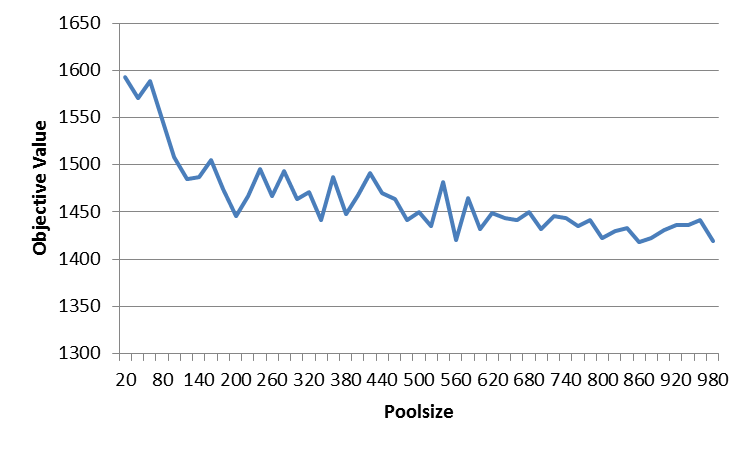
\includegraphics[height=6cm]{OVP}
\caption{\textsl{The Objective Value vs. The Poolsize}}
\label{OVP}
\end{figure}

The actual graphing of the data generated can be seen in figure \ref{OVP} and it’s immediately very clear that the ‘objective value’ converges towards 1406 which is the already established optimal tour in this TSP. The noteworthy thing here is that an increase in poolsize has minimal effect on the expected objective value, but more on the spread of the points.




\par
Now let’s take a look at the graphing of the poolsize against the time taken. 
Figure \ref{CTP} follows a surprisingly smooth curve which clearly is not linear but it’s hard to tell what relation it does follow. The current guess is that it is a quadratic relation but this will be investigated in a program designed for curve-fitting.

\begin{figure}[h] 
	\centering
	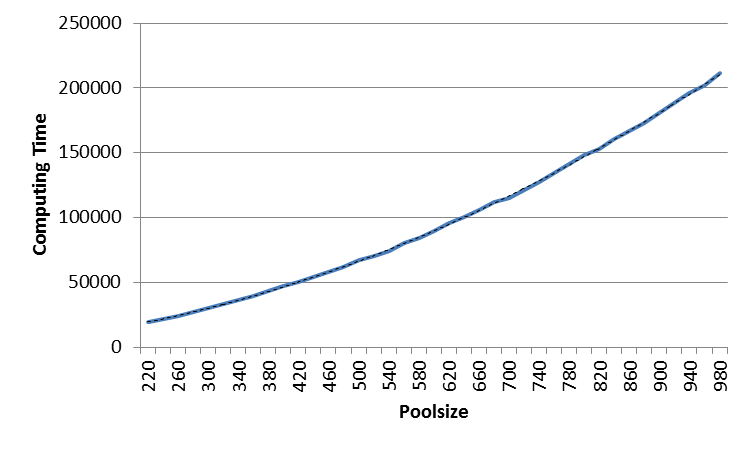
\includegraphics[height=6cm]{CTP}
	\caption{\textsl{The Computation Time vs. The Poolsize}}
	\label{CTP}
\end{figure}



\par
While the seemingly quadratic relation has not been proven via a logical statement using the properties of the code, it can be seen in figure \ref{LPPC} that the data so far does fit a quadratic relation very nicely. Maybe even more convincing is what happens in the next figure \ref{LPPP} where the curving-software is asked to predict the graph when only giving a very small part of it. The accuracy of this prediction is very convincing for the case of a quadratic relation and even though it could very well turn out to be a very weak 4th power relation, it is assumed to be quadratic and treated as such.

\begin{figure}[h] 
\centering
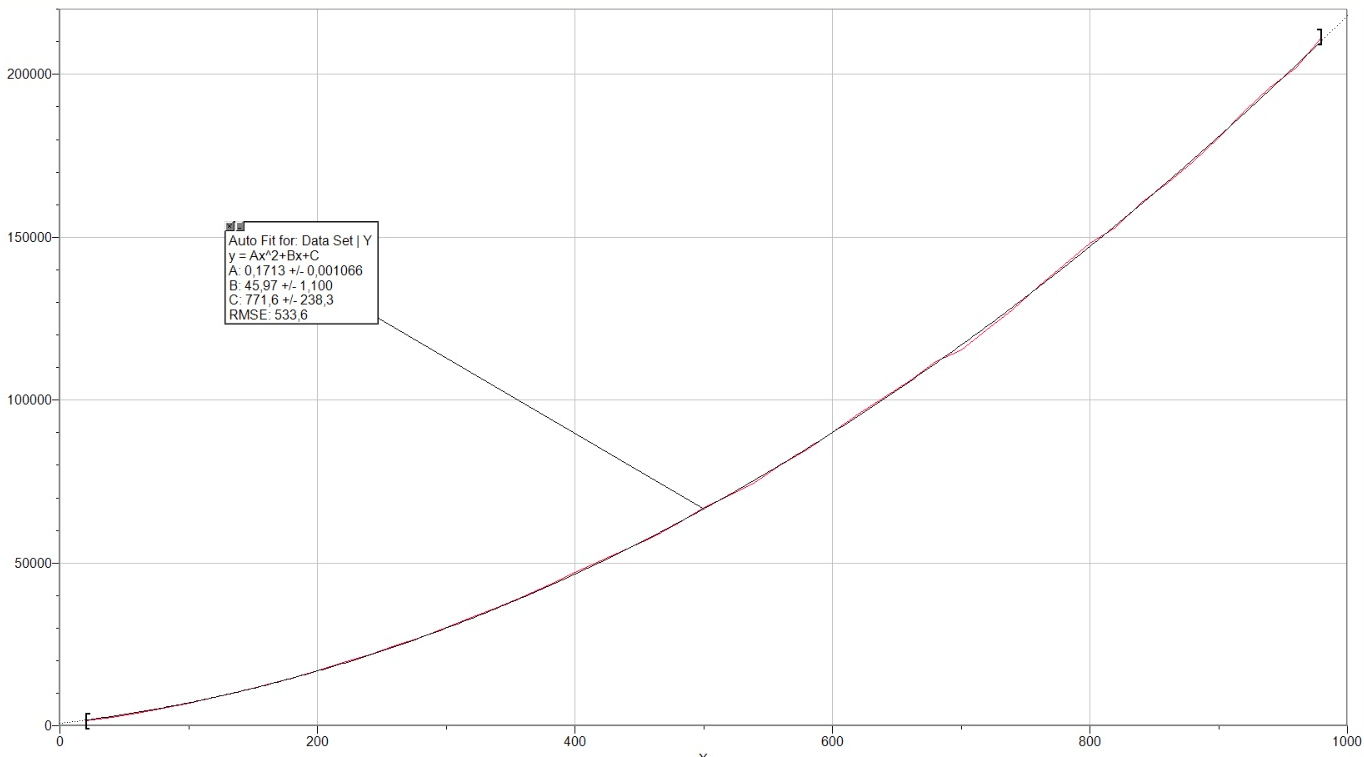
\includegraphics[height=6cm]{LPPC}
\caption{\textsl{The quadratic fit}}
\label{LPPC}
\end{figure}

\begin{figure}[h] 
\centering
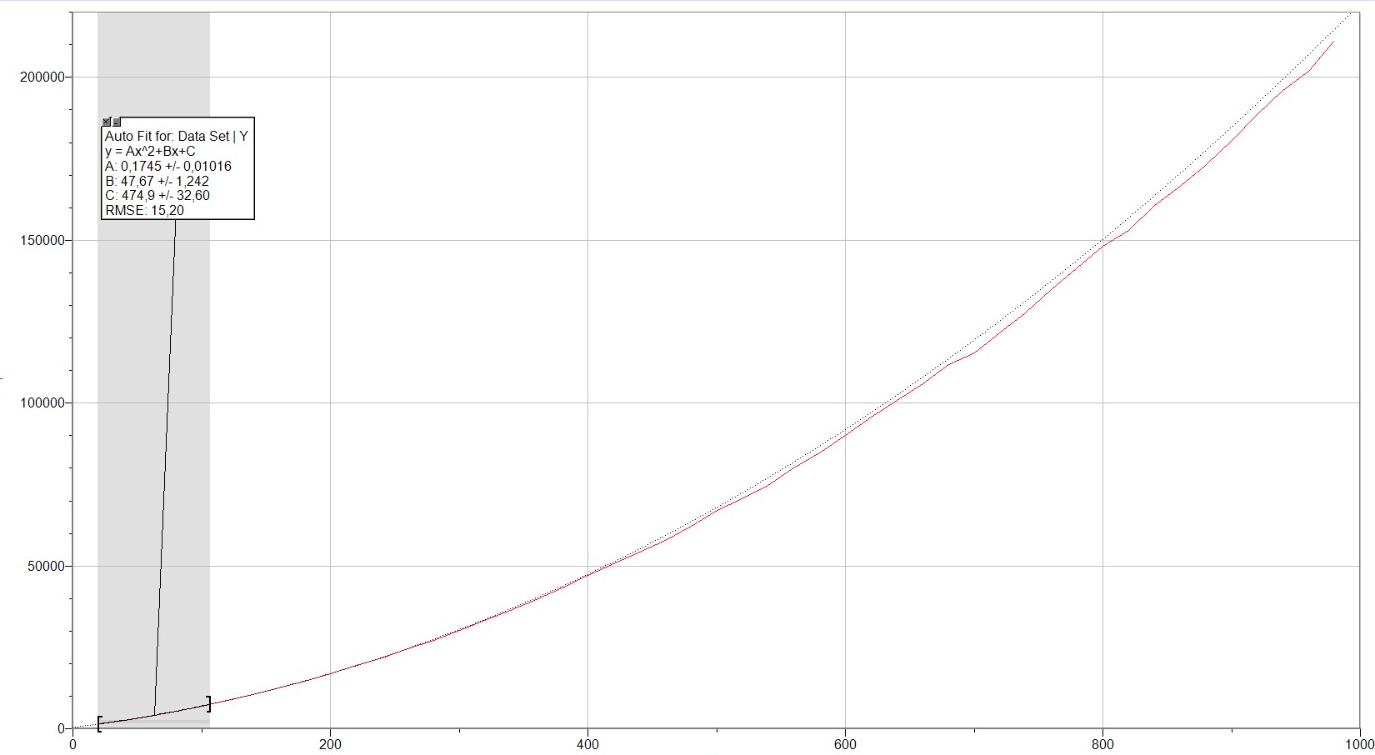
\includegraphics[height=6cm]{LPPP}
\caption{\textsl{The predicted fit}}
\label{LPPP}
\end{figure}

\par
A noteworthy property of these and the upcoming graphs is that they are very spiky, even after having taken an average. These spikes are in essence a reminder that the GA is a program that depends on randomness. Furthermore, the fact that the GA depends on randomness is exactly the reason why those spikes will never disappear. They might decline in amplitude and reduce their frequency, but since they are products of random events, their absence can never be guaranteed. Just like it will also be possible for any amount of coins to all toss heads, no matter how many there are.
\par
One way to reduce the spikes would be to repeatedly run the GA and consider the whole data-set instead of just a singular value. Another, more efficient way, is to optimize the input parameters. In the case of poolsize it can already be seen that an increase reduces the spikes in the objective value.

\subsection{The amount of generations}

\par
The way that the effect of the generations parameter has on the performances of the GA has been analysed much like that of the poolsize and the first part is the effects of changes in the amount of generations versus the the time spent computing of which the graph can be seen in figure \ref{CTG}.

\begin{figure}[h] 
	\centering
	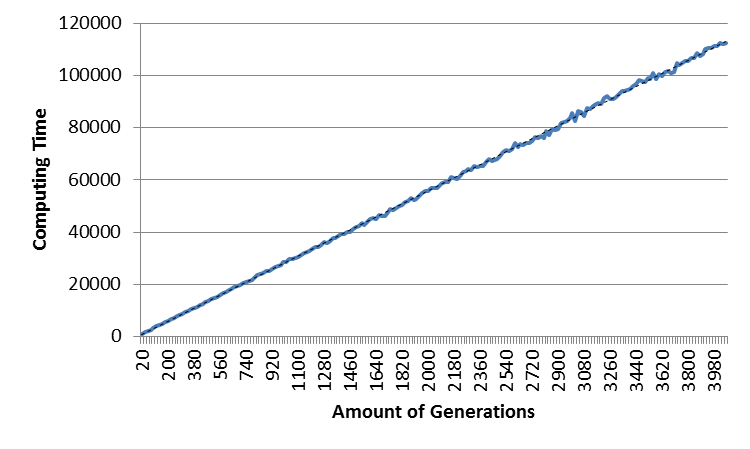
\includegraphics[height=6cm]{CTG}
	\caption{\textsl{The Computation Time vs. The amount of Generations}}
	\label{CTG}
\end{figure}

\par
The relation between the two can clearly be seen to be proportional. This makes sense intuitively since if the amount of generations would be doubled and the amount of calculations per generation would remain the same, then the total amount of calculations, and therefore the time needed to do the calculations, would double as well, and hence the linear relation.

The figure \ref{OVG} yields something interesting because, in contrary to the same graph of the poolsize, it does not reduce its spikes when the amount of generations increase.

\par
This can be explained by considering that after a certain point, the GA will have converged to some optimum and throwing more generations on it will not increase the chances of jumping to a better one. Instead the GA will stick with it’s found optimum for the whole of the extra added generations.


\begin{figure}[H] 
	\centering
	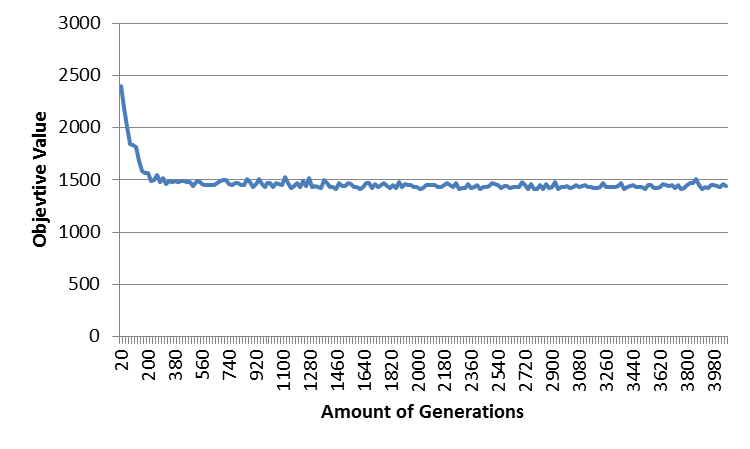
\includegraphics[height=6cm]{OVG}
	\caption{\textsl{The Objective Value vs. The amount of Generations}}
	\label{OVG}
\end{figure}



\subsection{The elites percentage}

\par
The effects of different values of the percentage of elites on the program have been analysed by considering how the computing time and the objective value behave and more specifically, the quality of the objective value and its standard deviation.

It can be seen in figure \ref{OVEP}  that the relation between the objective value and the elites percentage is quite stable. That is, if the outer edges are not considered because both extremes result in very poor convergence.

	\begin{figure}[h] 
		\centering
		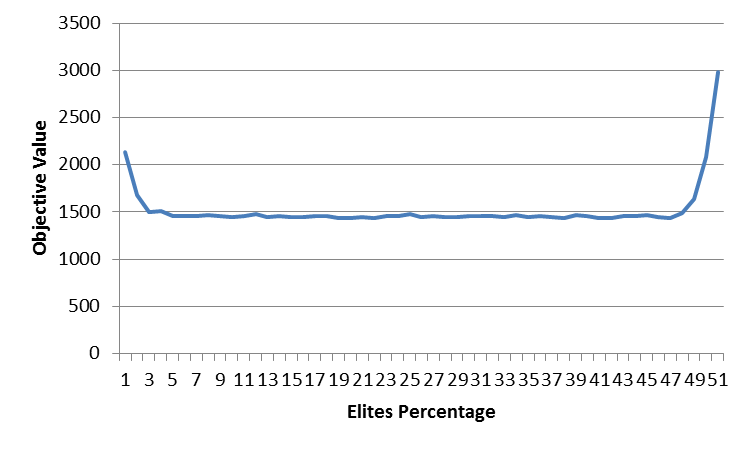
\includegraphics[height=6cm]{OVEP}
		\caption{\textsl{The Objective Value vs. The Percentage of Elites}}
		\label{OVEP}
	\end{figure}
	

\par 
The reason that the side with a too small elites percentage does converge significantly worse than that with other values for this parameter is because the program is effectively completely missing out on elites which are a vital part of the GA.
\par 
Then the question arises why it does not work with the higher values for the elites percentage and this is because the elites are not susceptible to change over the course of the generations. In other words, the GA barely gets to apply the very reason why the GA is even considered: a gradual increase of the quality of the solution over the course of many generations by combining and mutating the current generation.
\par
Figure \ref{CTEP} shows a linear but decreasing relation between the elites percentage and the computing time. This happens since the elites are not susceptible to change and therefore can the GA skip more and more of the computations the bigger the elites percentage becomes. So one should be careful about the illusion that a higher percentage of elites leads to a faster program. Instead the program simply does less calculations.

\begin{figure}[h] 
	\centering
	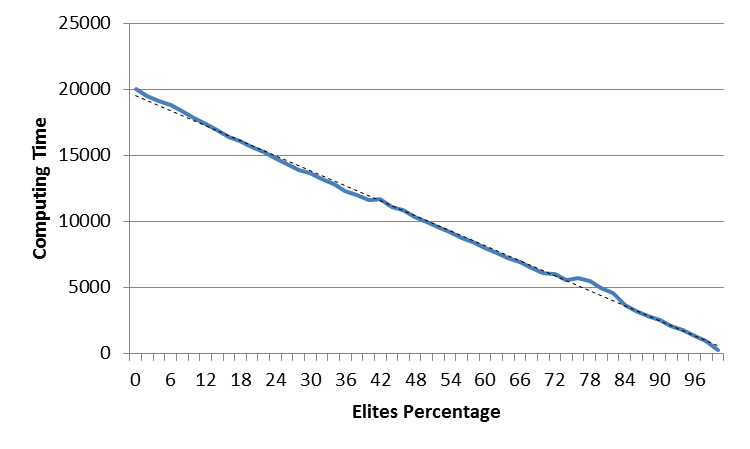
\includegraphics[height=6cm]{CTEP}
	\caption{\textsl{The Computation Time vs. The Percentage of Elites}}
	\label{CTEP}
\end{figure}

Finally, figure \ref{SDEP} shows the standard deviation of the objective value for different values of the elites percentages. It can be seen that the elites percentage obtains optimal consistency around 30 percent of the poolsize.

\begin{figure}[h] 
	\centering
	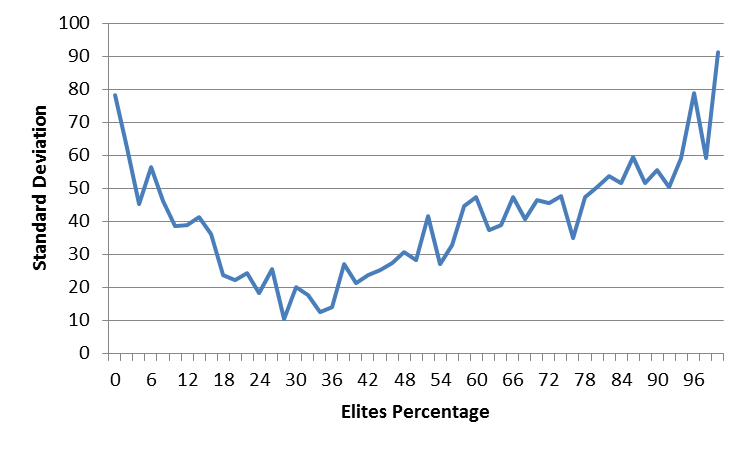
\includegraphics[height=6cm]{SDEP}
	\caption{\textsl{The Standard Deviation vs. The Percentage of Elites}}
	\label{SDEP}
\end{figure}




\subsection{The Rate of Mutation}
When considering the rate of mutation in the program, it is intuitively clear that this will have a minimal effect on the time needed to get the solution but it might deliver more interesting effects on the objective value and its standard deviation.
The statement about the time needed can quickly be verified with figure \ref{CTRM}, and indeed there it can be seen that there is not a notable effect on the computation time.

\begin{figure}[h] 
	\centering
	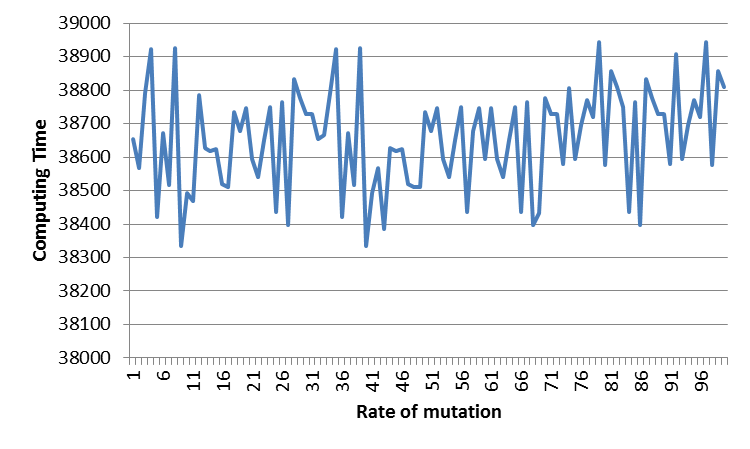
\includegraphics[height=6cm]{CTRM}
	\caption{\textsl{The Computation Time vs. The Rate of Mutation}}
	\label{CTRM}
\end{figure}


\par
In figure \ref{OVRM}, the plotting of the objective value versus the rate of mutation can be found, and it can be seen that there seems to be a very slight decreasing factor in there. But more notably is the little dip it attains around a rate of mutation of 30 percent. It does not look like much but it should be kept in mind that the minimum this graph could ever obtain is 1406. and since this little dip comes consistently close to that particular value it is a very significant drop.

\begin{figure}[h] 
	\centering
	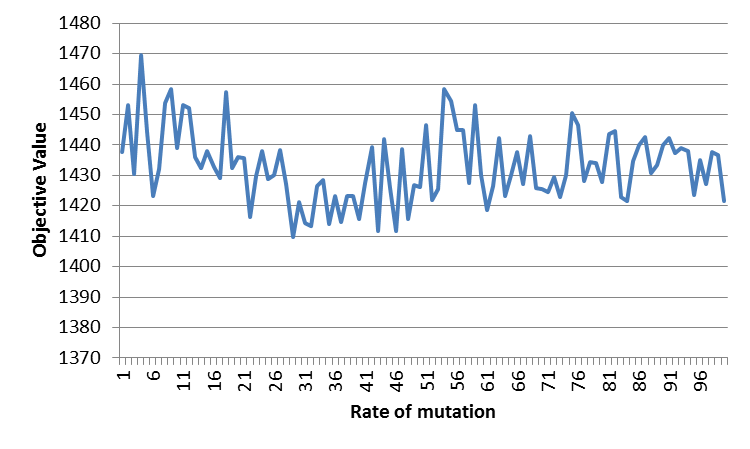
\includegraphics[height=6cm]{OVRM}
	\caption{\textsl{The Objective Value vs. The Rate of Mutation}}
	\label{OVRM}
\end{figure}

The drop around the 30 percent mark can perhaps better be considered in Figure \ref{SDRM} concerning the standard deviation versus the rate of mutation, and much like the previous graph there is a very notable drop around this value for the rate of mutation. The existence of this dip also immediately explains the dip in the previous graph since the program tries to get to 1406 all the time, but at these values it can do so more consistently hence the lower average of the objective value.
\par

\begin{figure}[h] 
	\centering
	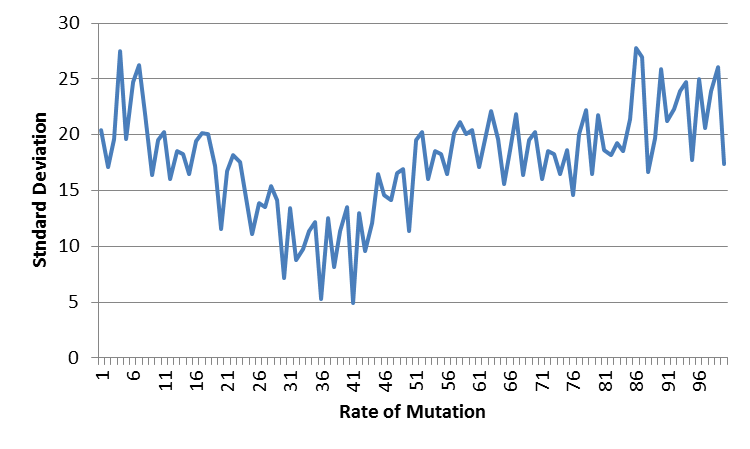
\includegraphics[height=6cm]{SDRM}
	\caption{\textsl{The Standard Deviation vs. The Rate of Mutation}}
	\label{SDRM}
\end{figure}

\subsection{Conclusions of the analysis}

\par
At the beginning of the this chapter, three main properties were mentioned to be judged: The time taken to finish, the actual quality of the objective value and its consistency.
\par
After having seen all the graphs and relations so far, some conclusions can be made with respect to preferable settings for the optimal experience while handling the GA.
For starters, to gain access to the better solutions in the solution space, it is recommended to invest in both the poolsize and the amount of generations to overcome the threshold both of those parameters have at the lower values. Furthermore, the elites percentage should not be in either of its extreme ends for this goal.
\par
If the goal is to increase the potency of the GA while limiting the extra added time needed to finish, it is recommended to invest in the poolsize up until the slope of the quadratic relation catches up to that of the amount of generations and from there invest in the generations. This will be especially effective in bigger problems since for smaller problems chances are that there is no need to be careful about the time needed since it is negligible anyway.
\par
Finally, considering the consistency of the GA, it already has been mentioned that both the elites percentage and rate of mutation give optimal consistency around a value of 30. Additionally, considering the poolsize and the amount of generations the standard deviation of those parameters are shown in the figures \ref{SDG} and \ref{SDP}. And it should be clear through the spikiness of the graphs that the standard deviation related to the amount of generations is generally constant in contrary to that of the poolsize since that seems to generally be decreasing. This means that the recommended settings for the goal of increasing the consistency can be concluded to be a minimal investment in the generations, a value between 30 and 50 for the elites percentage and a poolsize as big as the available computational power allows.

\begin{figure}[h] 
	\centering
	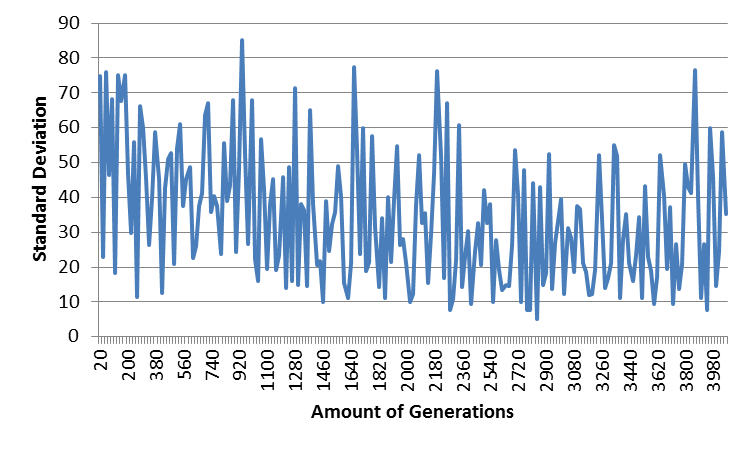
\includegraphics[height=6cm]{SDG}
	\caption{\textsl{The Standard Deviation vs. The amount of Generations}}
	\label{SDG}
\end{figure}

\begin{figure}[h] 
	\centering
	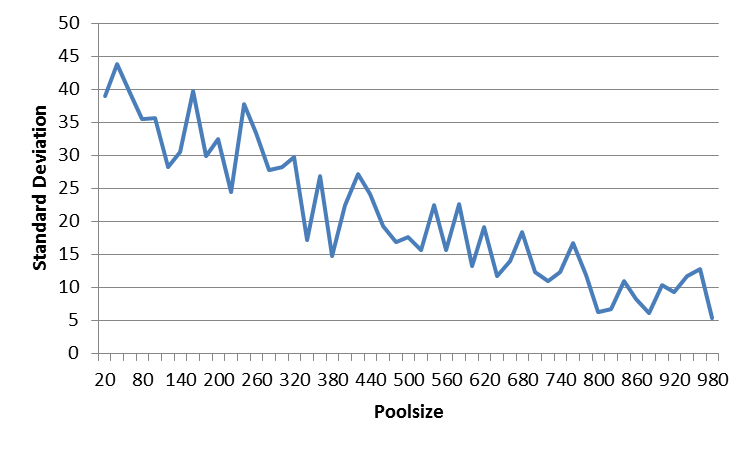
\includegraphics[height=6cm]{SDP}
	\caption{\textsl{The Standard Deviation vs. The Poolsize}}
	\label{SDP}
\end{figure}


